%%
%%
%%      SECTION: MAIN BEAM 
%%
%%__________________________________________________________________
\section{Main beam}% {\color{YellowGreen} Laurence $\&$ Jean-Fran\c cois}}
\label{se:MB}


We define NIKA2 main beam as the principal Gaussian (of the smaller FWHM)
that encloses most of the measured source flux. The best-fitting value
of the first Gaussian function of the
three-Gaussian model, as discussed in Sect.~\ref{se:fullbeam_prof},
provides us with a first estimate of the main beam. %, which is given in
%Table~\ref{tab:fwhm}.
However, this estimate could be biased toward the lower FWHM values due to
degeneracies between the three-Gaussian model parameters. To ensure
obtaining robust main beam FWHM estimates, we devise %
% version without JFL method
%an alternative dedicated method, which resorts to a mask of the side
%lobes and is described in Sect.~\ref{se:sidelobe_masked_method}.
% version including JFL method
two alternative dedicated
methods, which both resort to masking the side lobes: i) Gaussian fits
of the beam profile to benefit from the signal-to-noise ratio increase
after azimuthally averaging the signal, ii) Elliptical Gaussian fits
of the beam map for a better 2D modeling.
Cross-checking the outputs from these complementary methods is an
important robustess test of our results.

We also consider different data sets acquired during the N2R9
commissioning campaign and the N2R12 and N2R14 science pools: i) a
series of $8' \times 5'$ OTF scans of primary and secondary
calibrators, as described in Sect.~\ref{se:mb_with_otf}, ii)
\bm\ scans of bright sources, as discussed in
Sect.~\ref{se:mb_with_beammap}.


%\subsection{Sidelobe-masked Profile-based analysis}
%{\bf add a description here [Jean-Francois's method]}

\subsection{Sidelobe-masked 1D method}% {\color{YellowGreen} Jean-Fran\c cois}}
\label{se:beam_mb_1D} 

The brigthness radial profiles of a primary calibrator (Uranus or
Neptune) are first computed from their maps with a fine resolution
($1''$ pixel). Then a single Gaussian is fit to each profile after
masking data points at radial distances comprised between
$0.65 \times$ FWHM and $80''$, so that the error beam (side lobes)
does not bias the fit. In this approach, the data points at radial
distance beyond $80''$ provide the base level of the Gaussian fit. In
practice, maps $600'' \times 600''$ in size were made but only the
inner part within a radius of $180''$ with uniform rms was used to
compute the profile.
The best-fitting FWHM of the Gaussian model
yields the main beam FWHM for each array, as reported in Table
\ref{tab:fwhm}.

All \bm\ and shallower OTF scans of Uranus and Neptune in the N2R9,
N2R12 and N2R14 observation campaigns were used to determine the means
and standard deviations of the main beam fwhms for the three arrays in
Table~\ref{tab:fwhm}.



\subsection{Sidelobe-masked 2D method}% {\color{YellowGreen} Laurence}}
\label{se:beam_mb_2D}

\subsubsection{Method desciption}
\label{se:2D_method}

NIKA2 main beam two-dimensionnal distribution is modeled using an
elliptical Gaussian. We characterize NIKA2 resolution by forming the
\emph{FWHM}, defined as
\begin{equation}
  FWHM = 2 \sqrt{2\ln {2}} \sqrt{\sigma_x\sigma_y},
\end{equation}
where $\sigma_x$ and $\sigma_y$ are the Gaussian standard deviation
along minor and major axis.
To avoid the side lobes contamination, we use masked versions of the
beam map. The sidelobe mask consists in cutting an annulus of inner radius
$r_{\rm{in}}$ and outter radius $r_{\rm{out}}$ centered on the beam
maximum. Whereas $r_{\rm{out}}$ is conservately set to be $100''$,
$r_{\rm{in}}$ is let free to vary around a central value about $8''$
for A1 and A3 and about $12''$ for A2 to provide the best 2D Gaussian
fit.

\subsubsection{OTF scan based results}
\label{se:mb_with_otf}

\begin{figure}[ht!]
\begin{center}
  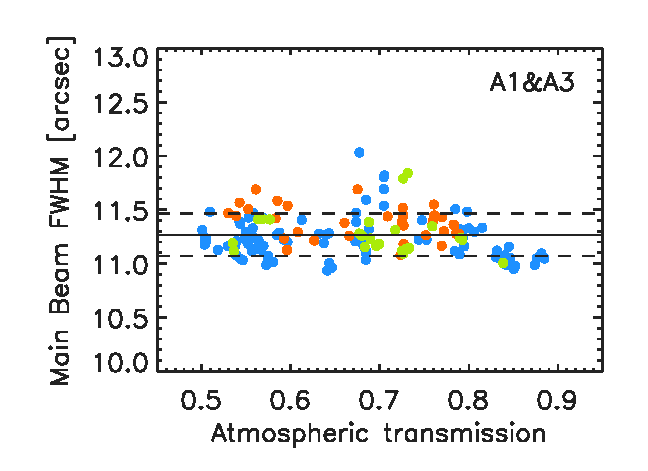
\includegraphics[clip, width=0.45\textwidth]{Figures/Beams/plot_FWHM_vs_atmtrans_mb_radius_binning2_1mm.pdf}
  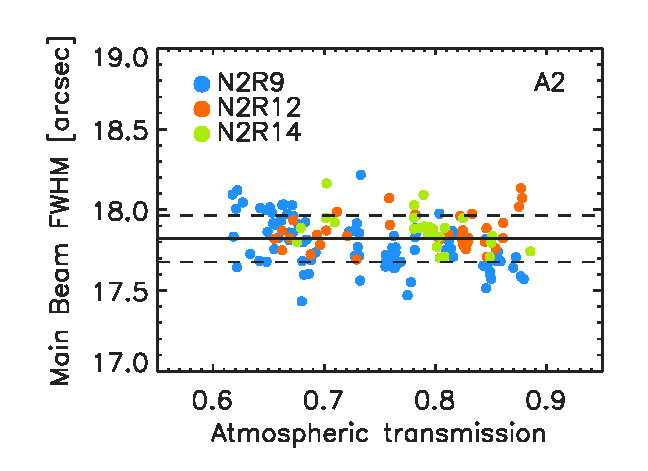
\includegraphics[clip, width=0.45\textwidth]{Figures/Beams/plot_FWHM_vs_atmtrans_mb_radius_binning2_a2.pdf}
  \caption[Main Beam FWHM]{Main beam FWHM estimates for the $1\,\rm{mm}$ (left) and $2\,\rm{mm}$ (right) channels are shown as a function of the atmospheric transmission using bright source scans acquired during N2R9, N2R12 and N2R14. }
\label{fig:fwhm_map_atmtrans}
\end{center}
\end{figure}

We select scans of moderately bright to very bright point sources by
thresholding the flux density estimates at $1~\rm{Jy}$ at both
wavelenths. Slightly extended sources, such as Mars, NGC7027 and
CRL2688 are discarded. After the baseline selection cuts, as described in
Sect.~\ref{se:data_selection}, the data set comprizes 163 scans
towards the giant planets Uranus and Neptune, the secondary calibrator
MWC349 and the quasars 3C84, 3C273, 3C345 and 3C454 (aka
2251+158). The data are reduced using the pipeline described in
Sect.~\ref{se:pipeline_overview} and projected onto $2''$ resolution
maps. The FWHM of the main beam is estimated following the
sidelobe-masked 2D method, as described in Sect.~\ref{se:2D_method}.
For Uranus, the
FWHM estimates are further corrected for the beam broadening due to the
extension of the apparent
disc. At the IRAM $30\,\rm{m}$ latitude, Uranus disc diameter varies
from $3.3''$ to $3.7''$. This induces a broadening of the Gaussian main beam of
$0.19 \pm 0.03\,\rm{arcsec}$ at 1-mm and $0.12 \pm 0.02\,\rm{arcsec}$
at 2-mm. Uranus FWMH estimates are corrected for the average beam
widening values.

Figure~\ref{fig:fwhm_map_atmtrans} shows the main beam FWHM estimates
as a function of the atmospheric transmission, which is modeled as
$\exp{\left(-\tau \cdot x\right)}$, where $\tau$ is the zenith opacity estimate and
$x$ the airmass, which is evaluated as the cosecant of the observing
elevation. The FWHM estimates using data of the three campaigns are in
agreement within rms errors. Moreover, the main beam FWHM is stable
against the atmospheric condition at both wavelengths. Slightly lower
values than average (about $11''$) are observed in the best
atmospheric conditions at $1\,\rm{mm}$ providing us with a lower limit
in the absence of correlated atmospheric noise residuals. We note
three scans acquired during N2R12 with larger FWHM than average at
$2\,\rm{mm}$ although the atmospheric transmission was excellent: this
is likely an effect of the abnormalous refraction, which impacted
a lot of scans during the N2R12 campaign. 

The distributions of the best-fitting FWHM values of array 1, 3, the
combination of arrays $1\&3$ and array 2 using the OTF scans from the
three observation campaigns are shown in Fig.~\ref{fig:fwhm_map}. Nine
scans with outlier $r_{\rm{in}}$ values have been discarded.
We checked a posteriori that $r_{\rm{in}}$
distributes as $10 \pm 1$ arcsec at $1\,\rm{mm}$ and $11 \pm 1$ arcsec
at $2\,\rm{mm}$. The average FWHM estimates and the rms errors are
reported in Table~\ref{tab:fwhm}.  


\begin{figure}[ht!]
\begin{center}
  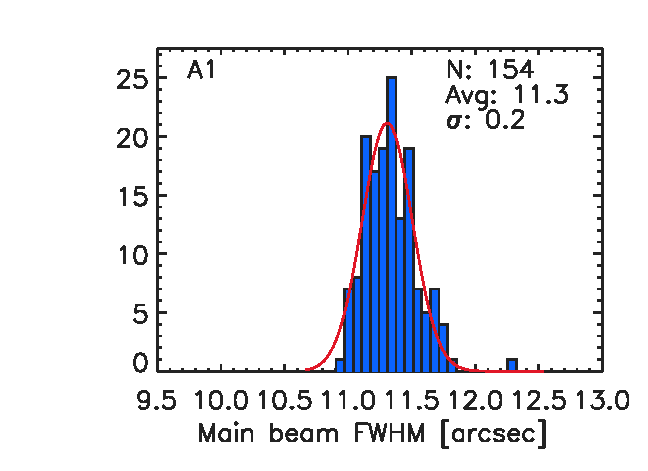
\includegraphics[clip, width=0.42\textwidth]{Figures/Beams/plot_histo_FWHM_mb_radius_binning2_a1.pdf}
  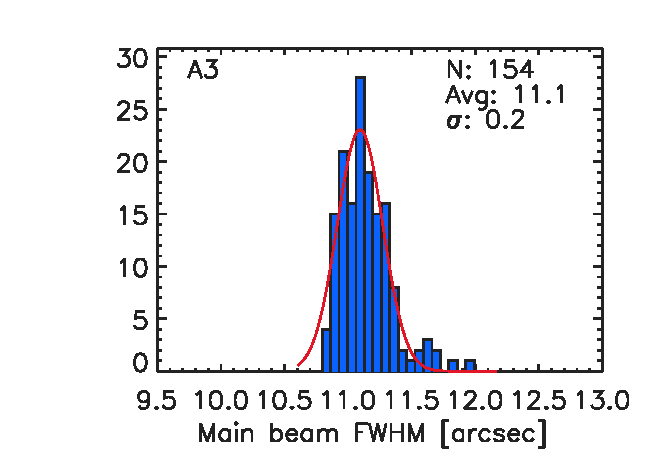
\includegraphics[clip, width=0.42\textwidth]{Figures/Beams/plot_histo_FWHM_mb_radius_binning2_a3.pdf}
  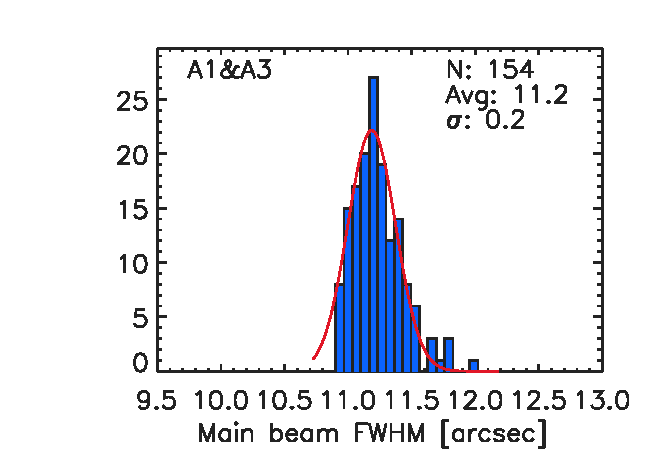
\includegraphics[clip, width=0.42\textwidth]{Figures/Beams/plot_histo_FWHM_mb_radius_binning2_1mm.pdf}
  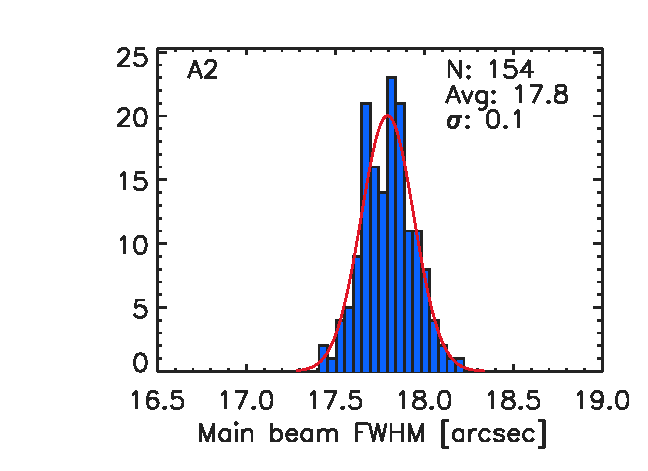
\includegraphics[clip, width=0.42\textwidth]{Figures/Beams/plot_histo_FWHM_mb_radius_binning2_a2.pdf}
  \caption[Main Beam FWHM distributions]{Distribution of the FWHM estimates for Array 1, 3, the combination of Array $1\&3$ and Array 2, including bright source scans from the three campaigns.}
\label{fig:fwhm_map}
\end{center}
\end{figure}

\subsubsection{Beammap scan based results}
\label{se:mb_with_beammap}

We select a sub-set of the \bm\ scan selection described in
Sect.~\ref{se:beammap_set} by discarding scans of Mars.
The 12 remaining \bm\ scans are analysed using the data reduction
pipeline of Sect.~\ref{se:pipeline_overview} and projected onto maps
with a resolution of $1''$ and an angular size of $10'$.    
The main beam FWHM is estimated using the sidelobe-masked 2D method, as
described in Sect.~\ref{se:2D_method}. Sidelobe masks are
defined by a fixed external radius $r_{\rm{out}}$ of $100''$ and a
fixed internal radius $r_{\rm{in}}$ of $8.5''$ at $1\,\rm{mm}$ and
$13.5''$ at $2\,\rm{mm}$. We checked we obtain compatible results when
$r_{\rm{in}}$ is let to freely varies from $8'$ to $10'$ at
$1\,\rm{mm}$ and from $10'$ to $14'$ at $2\,\rm{mm}$. The fixed
$r_{\rm{in}}$ values correspond to the average best-fitting
$r_{\rm{in}}$ of the free-$r_{\rm{in}}$ analysis. The main beam FWHM
estimates using the sidelobe-masked 2D method on the \bm\ scans are
gathered in Table~\ref{tab:fwhm}.


\subsection{Comparison of the main beam FWHM estimates}
\label{se:fwhm_results}

We have derived the main beam FWHM for the three array and the
$1\,\rm{mm}$ array combination using three methods and three data
sets. Namely, our main beam FWHM estimates
consist of i) the median FWHM of the first (lowest-FWHM) Gaussian
function within the three-Gaussian model fitted from the 12 \bm\ scan
sub-set described in
Sect.~\ref{se:mb_with_beammap}, ii) the average FWHM using the
sidelobe-masked 1D method on a series of \bm\ and $5'x8'$ OTF scans of
Uranus and Neptune, the sidelobe-masked 2D method average FWHM
from iii) a series of $5'x8'$ OTF scans of bright point sources and
iv) from the 12 \bm\ scan sub-set. The results of these analysis are
gathered in Table~\ref{tab:fwhm}, including error bars evaluated as
the rms dispersion of single-scan based FWHM estimates.

All the tests based on sidelobe-masked methods yield FWHM estimates
in agreement within error bars, whereas the test resorting to the
three-Gaussian model yields slightly smaller FWHM for all arrays. The
latter provides us with lower limits for the main beam FWHM. The error
bars are the most robustly derived from the dispersion of the
best-fitting FWHM over the set of 154 OTF scans, whereas rms errors
that are estimated from smaller scan sets are likely to be
underestimated. The combined results are obtained from an error-weighted
average of the four FWHM estimates for each array. The 12 \bm\ scan
based rms errors were replaced by the 154 OTF scan based rms errors
beforehand.
The combined FWHM estimates are given in Table~\ref{tab:fwhm}.

\begin{table}[h]
  \caption[]{FWHM of the NIKA2 main beam in arcsec.}
  \centering
  \begin{threeparttable}
  \begin{tabular}{|l|c|c|c|c|c|}
    \hline
    
       &    &  \multicolumn{4}{|c|}{Array or array combination} \\
    \cline{3-6}
    Method & Dataset        &   A1 &  A3 & A1 $\&$ A3 &  A2  \\
    \hline
    \hline
    Three-Gaussian model G1\tnote{a} &  \bm\     & $10.8 \pm 0.1$  &  $10.8 \pm 0.1$  & $10.8 \pm 0.1$  &  $17.4 \pm 0.1$  \\
    Sidelobe-masked 1D method        &  mixed    & $11.3 \pm 0.4$  &  $11.2 \pm 0.4$  & $11.2 \pm 0.3$   & $17.4 \pm 0.2$  \\ 
    Sidelobe-masked 2D method        &  5x8 OTF  & $11.3 \pm 0.2$  &  $11.1 \pm 0.2$  & $11.2 \pm 0.2$  &  $17.8 \pm 0.1$  \\ 
                                     &  \bm\     & $11.2 \pm 0.1$  &  $11.1 \pm 0.1$  & $11.2 \pm 0.1$  &  $17.6 \pm 0.1$  \\
    \hline
    \multicolumn{2}{|c|}{Combined}               & $11.1 \pm 0.2$  &  $11.0 \pm 0.2$  & $11.1 \pm 0.2$  &  $17.6 \pm 0.1$  \\
    \hline
  \end{tabular}
  \begin{tablenotes}
  \item[(a)] Median FWHM of the first (lowest-FWHM) Gaussian function
    within the Three-Gaussian model fitted from 12 \bm\ scans 
  \end{tablenotes}
  \end{threeparttable}
  \label{tab:fwhm}
\end{table}



\subsection{FWHM distribution across the FoV}
\label{se:fwhm_fov}

% COPY FROM THE 'INSTRUMENT' PAPER
\begin{figure}[ht!]
  \centering
  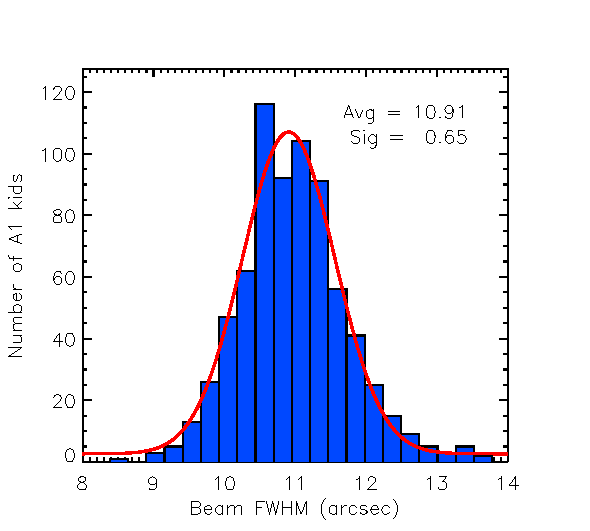
\includegraphics[clip=true,width=0.45\textwidth]{Figures/Papier2017/plot_histo_A1_fwhm_20170424s123.pdf}
  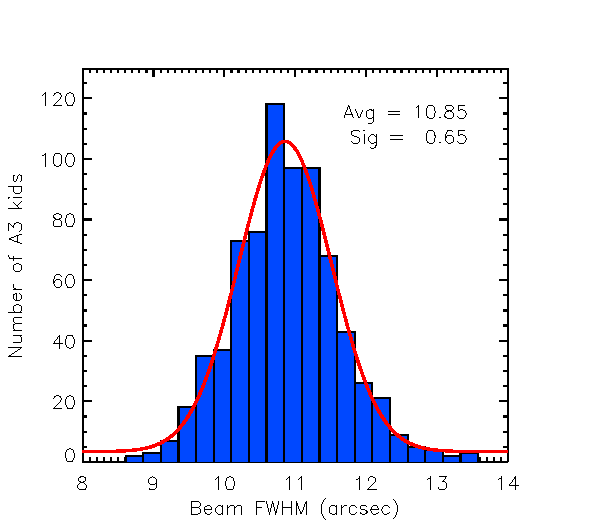
\includegraphics[clip=true,width=0.45\textwidth]{Figures/Papier2017/plot_histo_A3_fwhm_20170424s123.pdf}
  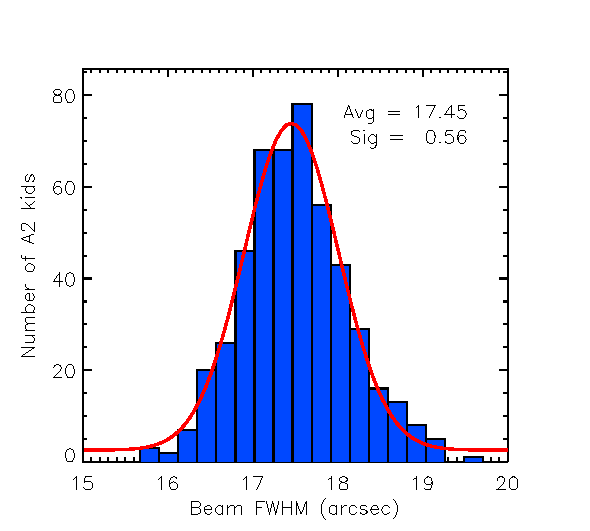
\includegraphics[clip=true,width=0.45\textwidth]{Figures/Papier2017/plot_histo_A2_fwhm_20170424s123.pdf}
  
\caption[Main beam FWHM distribution across the array]{Main beam FWHM distribution of all valid KID detectors of arrays A1, A3, and A2. The main beam FWHM is the geometrical combination of the two-orthogonal FWHM estimates obtained from an elliptical Gaussian fit on side-lobe masked individual maps per KID using a \bm\ scan of N2R9 (scan ID: 20170424s123). The red curves show a Gaussian fit to the histogram data.}
  \label{fig:focalplane_histo}
\end{figure}

Figure \ref{fig:focalplane_histo} shows the distribution of the
main beam FWHMs of the arrays A1, A3 and A2 using a beammap
scan of Neptune acquired during the April 2017 commissioning
campaign and for average weather conditions (scan ID: 20170424s123).
We also
show in red the best Gaussian fit to histogram data. We find an
average main beam FWHM of $10.9''$ at 260 GHz and $17.5''$ at
150 GHz in agreement with the main beam estimates gathered in
Table~\ref{tab:fwhm}.
The observed dispersion of about $0.6''$ is expected from the optics design and its associated
field distortions across the 6.5 arc-minutes FoV, as discussed in
Sect.~\ref{se:grid_distortion}. This quantifies the impact of the
non-constant focus across the FoV, which is characterised in
Sect.~\ref{sec:focus_surfaces}, on the individual detector main beams.  





